\documentclass[12pt]{article}
\usepackage{amscd,amssymb,amsthm,amsxtra,exscale,latexsym,verbatim,paralist}
\usepackage{mathrsfs}
\usepackage[T1]{fontenc}
\usepackage{newtxmath,newtxtext}
\usepackage[margin=1in]{geometry}

%\usepackage{mathtools}
%\usepackage{multicol}
\usepackage{tikz}

\pagestyle{empty} 
\setlength{\parindent}{0pt} 
\setlength{\parskip}{\baselineskip}

\theoremstyle{plain}
\newtheorem{ex}{Exercise}

\renewcommand{\proofname}{Solution}

%\makeatletter
%\renewcommand*\env@matrix[1][*\c@MaxMatrixCols c]{%
%  \hskip -\arraycolsep
%  \let\@ifnextchar\new@ifnextchar
%  \array{#1}}
%\makeatother

\begin{document}

MTH 385 \qquad 2022-02-23 Worksheet

\begin{ex}
  Recount the textbook's description of \emph{Gaussian elimination}.
\end{ex}

\begin{ex}
  Recount the textbook's description of elimination for simultaneous polynomial equations in two (or more) variables.
\end{ex}

\begin{ex}
  The textbook mentions Cramer's rule in passing. Describe Cramer's rule.
\end{ex}

\begin{ex} [5.2.1]
  Derive an equation that is linear in $y$ from the two equations
  \begin{align*}
    x^2+xy+y^2    &= 1, \\
    4x^2+3xy+2y^2 &= 3,
  \end{align*}
  and hence show that $y=(1-2x^2)/x$.
\end{ex}

\begin{center}
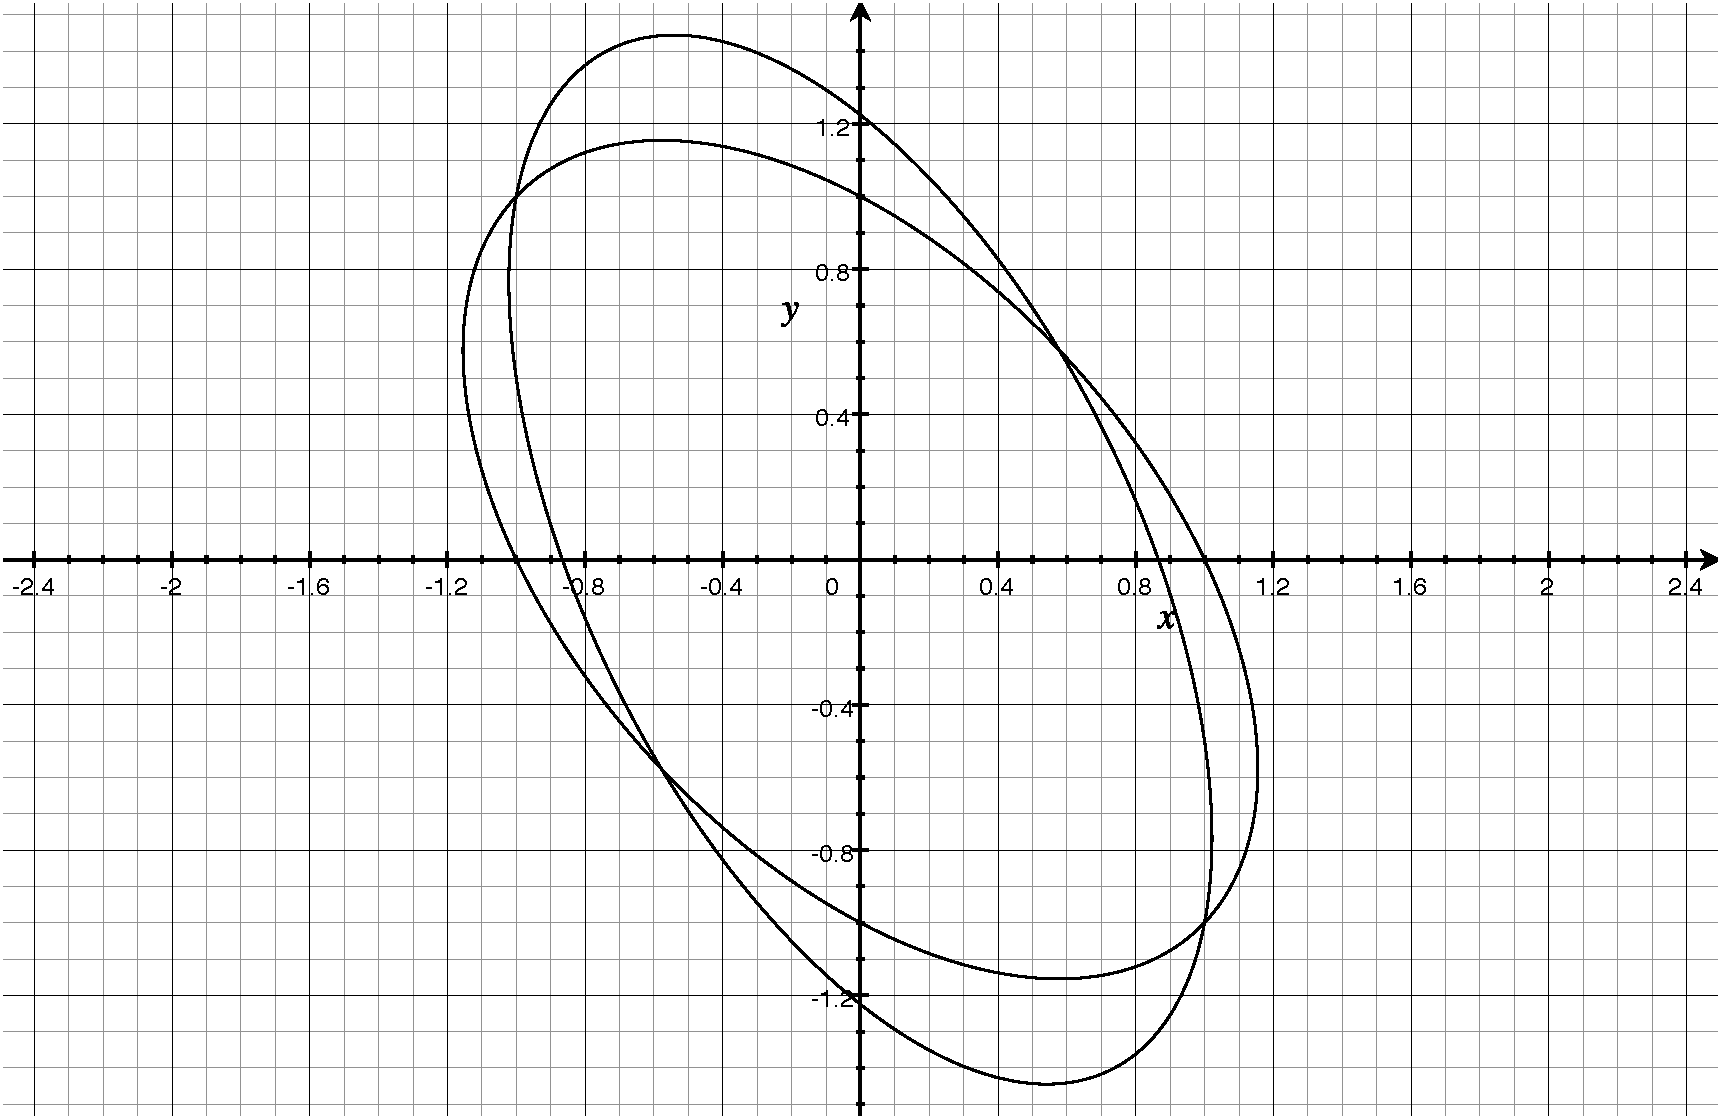
\includegraphics[scale=0.5]{curves}
\end{center}

\begin{ex} [5.2.2]
  Deduce that the intersections of the two curves in Exercise~5.2.1 occur where $x$ satisfies $3x^4-4x^2 +1=0$.
\end{ex}

This example, where the two equations of degree $2$ yield a single equation of degree $4(=2\times2)$, illustrates a general phenomenon where degrees are multiplied. We will observe other instances, and study it more deeply, as the book progresses.

The present example is not a typical equation of degree $4$, since it is quadratic in $x^2 = z$. However, this makes it a lot easier to solve.

\begin{ex} [5.2.3]
  Solve $3z^2-4z+1=0$ for $z=x^2$ by factorizing the left-hand side, and hence find four solutions for $x$.

  Give geometric reasons why you would expect two curves of degree $2$ to have up to four intersections. Could they have more than four?
\end{ex}

\end{document}

